\section{結果を描画する}
\label{sec:quicklook}
%####################################################################################

SCALEモデルの出力ファイルはMPIプロセス毎に出力されるため,
計算領域が分割された状態で出力される.
それぞれのファイルフォーマットは気候・予報(CF)メタデータ規約
に対応したnetcdf4形式である.
ここでは,プロセス毎に分割されたnetcdfファイルをgradsで扱うことがバイナリーファイルにまとめ、いくつか、確認のための図を示す.

\subsubsection{GrADSバイナリーに変換}
%-----------------------------------------------------------------------------------
分割されたnetcdfからGrADSバイナリー変換するには、\verb|netcdf2grads_h|を使用する.
詳細な使用方法は \ref{sec:net2g}節を参照頂きたい.

まず、\ref{sec:source_net2g}節でコンパイルしたバイナリーファイルにリンクを張る.
\begin{verbatim}
 $ ln -s ../../../../util/netcdf2grads_h/net2g ./
\end{verbatim}
ここでは例として、2次元変数であるMSLP、PRECを、
3次元変数として850hPa,500h,200hPa面のU、Vを変換する.
2次元変数のための設定は\verb|net2g.2d.conf|に、
3次元変数のための設定は\verb|net2g.3d.conf|にある.
configureの中のパラメータの設定は\ref{sec:net2g}節を参照頂きたい.

\verb|netcdf2grads_h|で使用可能なプロセス数は、
計算実行時に使用したプロセス数の約数である必要がある.
ここでは、計算に用いたのと同じ4ノード使用して変換することにする.
\begin{verbatim}
 $ mpirun -n 4 ./net2g net2g.2d.conf
 $ mpirun -n 4 ./net2g net2g.3d.conf
\end{verbatim}
成功すれば、下記のファイルが作成される.
\begin{verbatim}
  MSLP_d01z-2d.ctl
  MSLP_d01z-2d.grd
  PREC_d01z-2d.ctl
  PREC_d01z-2d.grd
  U_d01z-3d.ctl
  U_d01z-3d.grd
  V_d01z-3d.ctl
  V_d01z-3d.grd
\end{verbatim}


\subsubsection{計算結果の確認}
%-----------------------------------------------------------------------------------
現在のバージョンの\verb|netcdf2grads_h|では、
SCALEのXY格子座標でのみ、ctlファイルを作成可能である。
今後、緯度経度座標で出力できるようになる予定であるが、
作図の簡便さのために、下記の緯度経度座標で作図するためのctlを別途用意している.
\begin{verbatim}
  MSLP_d01z-2d_lcc.ctl
  PREC_d01z-2d_lcc.ctl
  U_d01z-3d_lcc.ctl
  V_d01z-3d_lcc.ctl
\end{verbatim}

計算結果確認用のサンプル図を作成するための
スクリプト\verb|checkfig.gs|を使って作図する.
\begin{verbatim}
 $ grads -blc checkfig.gs
\end{verbatim}
成功すると、下記の図が作成される.
なお、gradsのバージョンによって文法が異なるので、適宜変更する.
\begin{verbatim}
  mslp.png
  prec.png
  wind.png
\end{verbatim}
下記の図と同じであるか、答え合わせをする.

\begin{figure}[h]
\begin{center}
  \includegraphics[width=0.55\hsize]{./figure/real_mslp.eps}\\
  \caption{計算開始から12時間後の海面更正気圧}
  \label{fig:real_mslp}
\end{center}
\begin{center}
  \includegraphics[width=0.55\hsize]{./figure/real_prec.eps}\\
  \caption{計算開始から12時間後の1時間積算降水量}
  \label{fig:real_prec}
\end{center}
\begin{center}
  \includegraphics[width=0.55\hsize]{./figure/real_wind.eps}\\
  \caption{計算開始から12時間後の500hPaの風速と風ベクトル}
  \label{fig:real_wind}
\end{center}
\end{figure}



